%----------------------------------------------------------------------------
\chapter{Evaluation}
%----------------------------------------------------------------------------

%%----------------------------------------------------------------------------
%\section{Continuous Delivery}
%%----------------------------------------------------------------------------

%----------------------------------------------------------------------------
\section{Enhancements}
%----------------------------------------------------------------------------

%----------------------------------------------------------------------------
\subsection{Kafka}
%----------------------------------------------------------------------------

\begin{figure}[h]
	\centering
	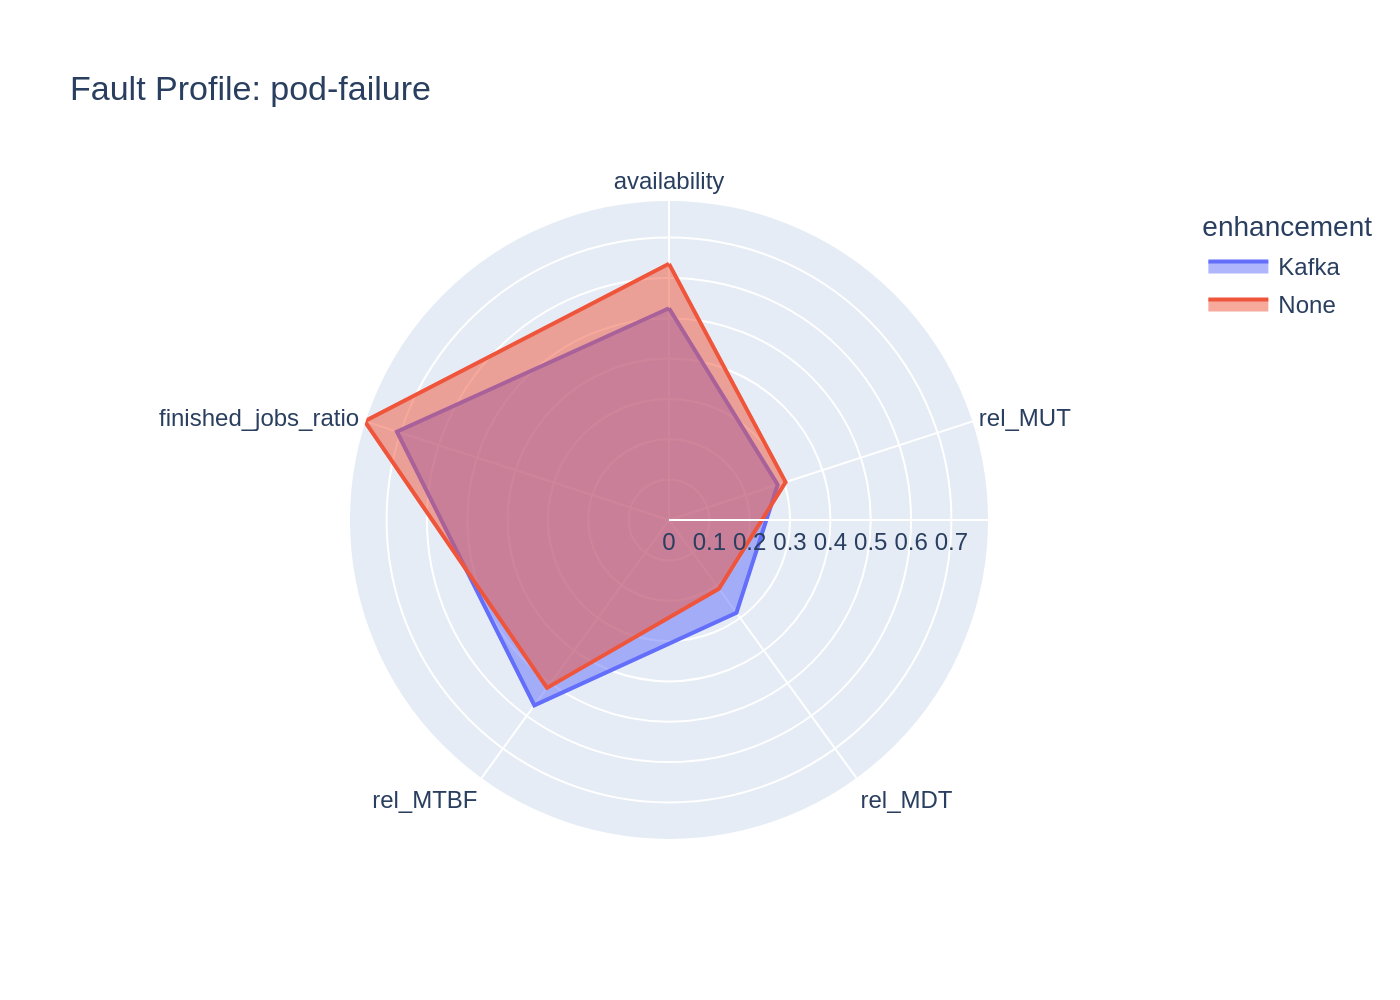
\includegraphics[width=140mm, keepaspectratio]{figures/kafka_with_base_pod-failure.png}
	\caption{Kafka enhancement - pod-failure fault profile}
	\label{fig:kafka-results-pod-failure}
\end{figure}

\begin{itemize}
	\item turns out, adding the complexity of kafka integration does not improve dependability metrics -- at least with the basic configurations (just Kafka and Zookeeper nodes 3-3 / 5-5), Kafka needs further components, hardening for robust operation -- log persistence (memory lost on pod-failure)
\end{itemize}

\begin{figure}[h]
	\centering
	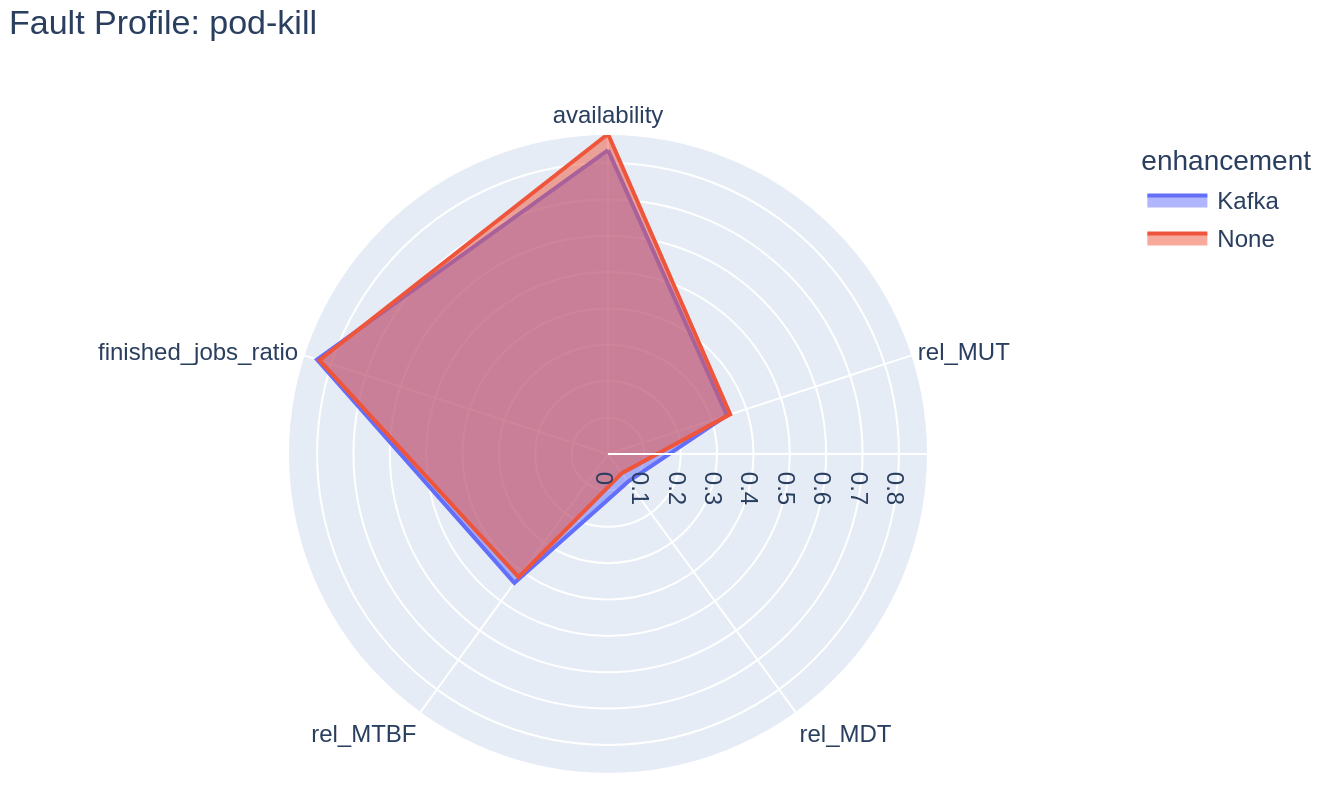
\includegraphics[width=140mm, keepaspectratio]{figures/kafka_with_base_pod-kill.png}
	\caption{Kafka enhancement - pod-kill fault profile}
	\label{fig:kafka-results-pod-kill}
\end{figure}

\begin{itemize}
	\item pod-kill scenario approximately is the same with Kafka (as described before, pod-kill is less severe than pod-failure chaos)
\end{itemize}

%----------------------------------------------------------------------------
\subsection{Heartbeats}
%----------------------------------------------------------------------------

\begin{itemize}
	\item the simple algorithm could improve the jobs ratio in both cases
	\item pod-kill was considerably better
	\item heartbeat is weak against backend of db downtime - but there are more worker components in average, so they are more likely to fail statistically -- improve: backend and db in HA
\end{itemize}

\begin{figure}[h]
	\centering
	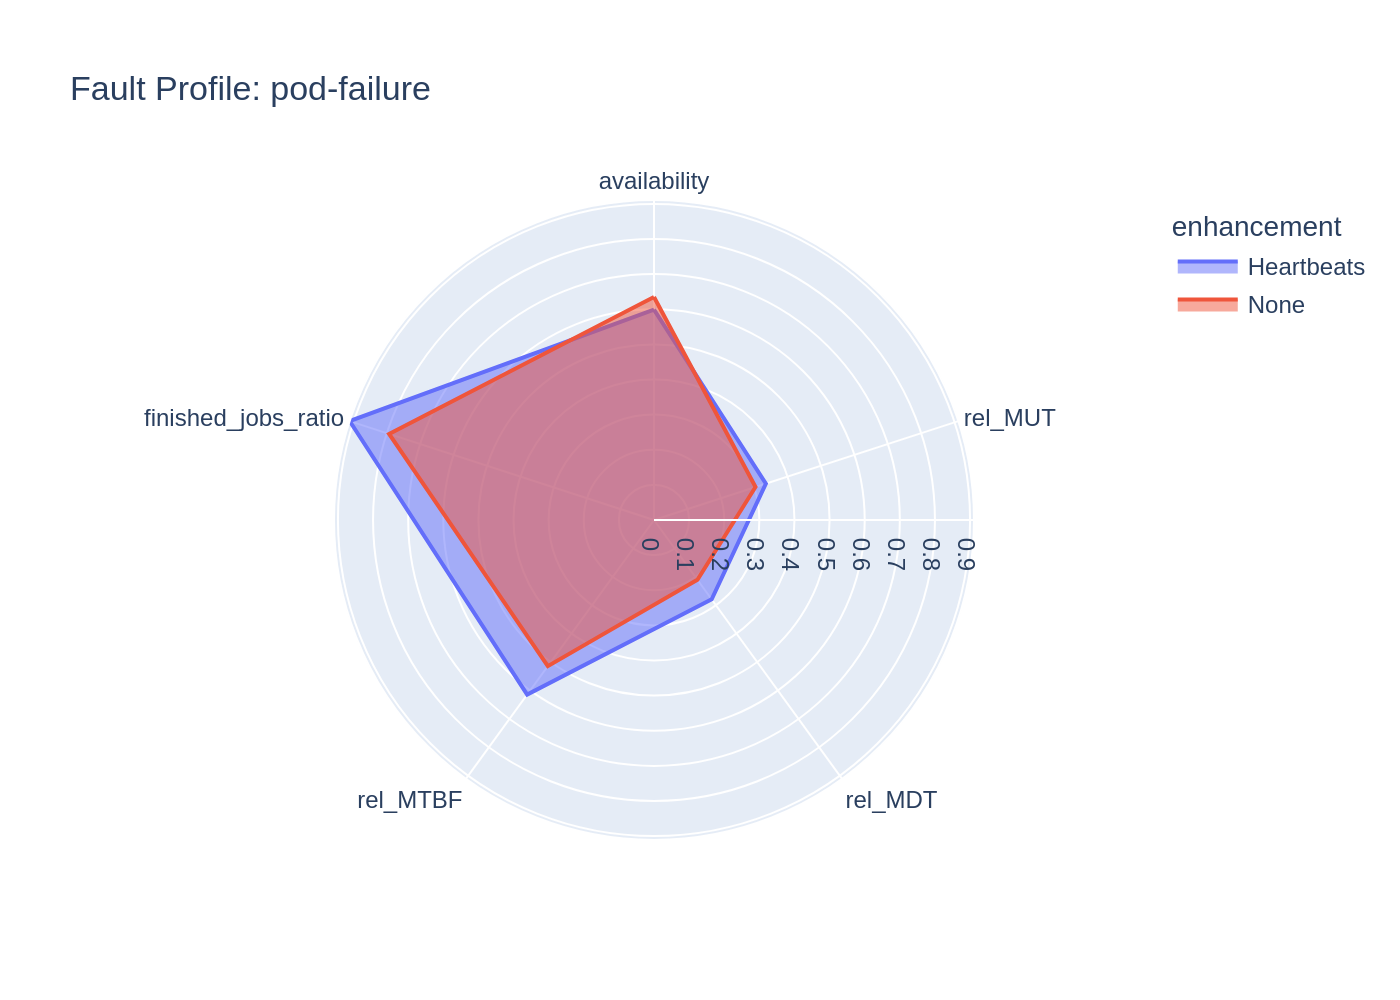
\includegraphics[width=140mm, keepaspectratio]{figures/heartbeats_with_base_pod-failure.png}
	\caption{Heartbeats enhancement - pod-failure fault profile}
	\label{fig:heartbeats-results-pod-failure}
\end{figure}

\begin{figure}[h]
	\centering
	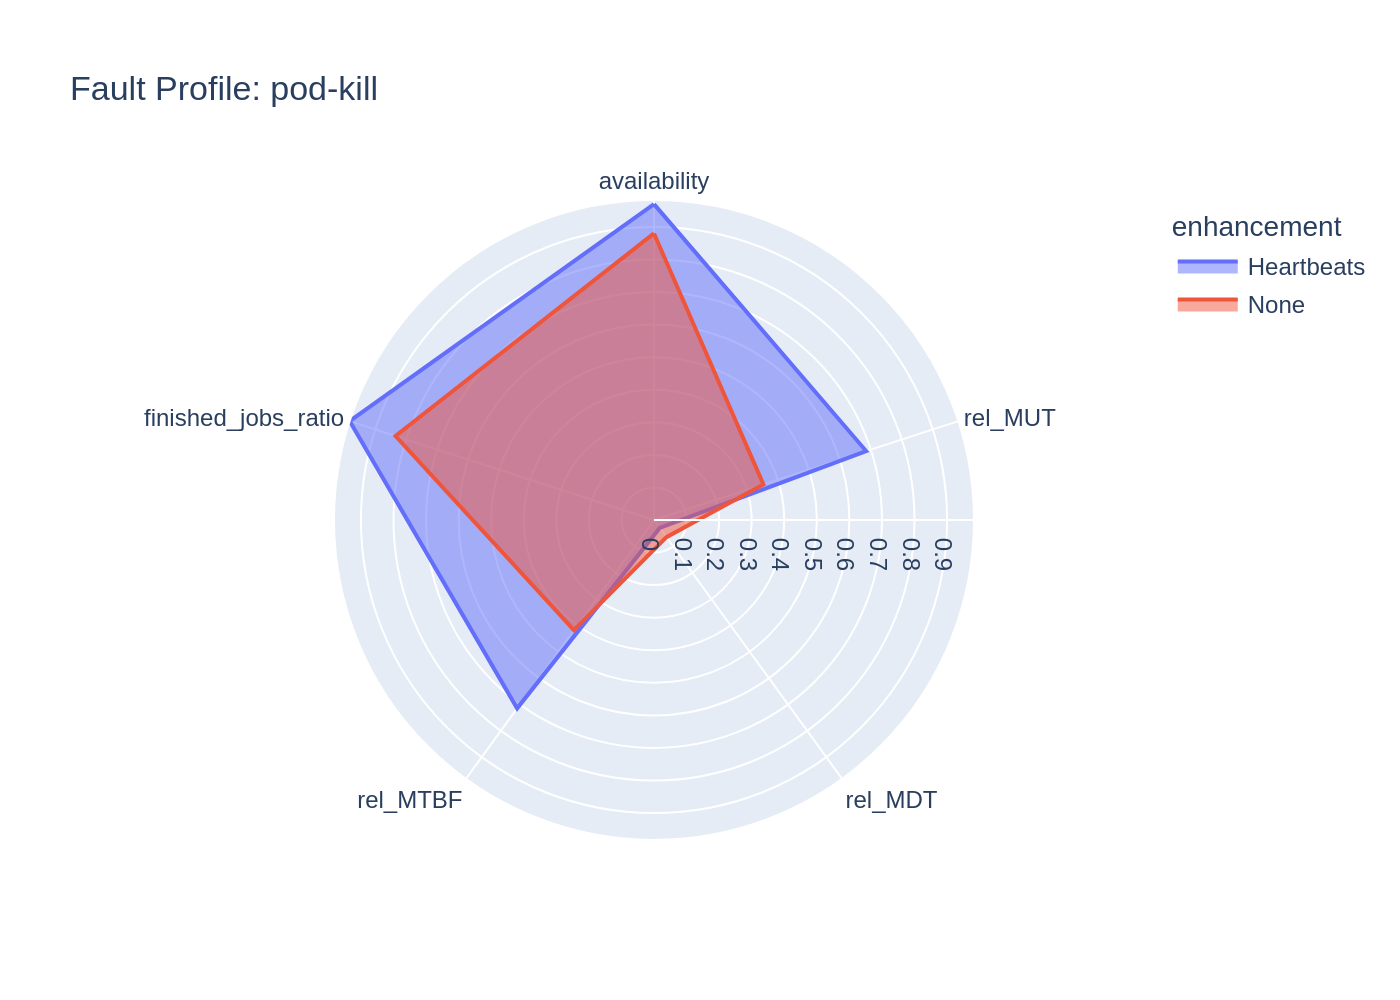
\includegraphics[width=140mm, keepaspectratio]{figures/heartbeats_with_base_pod-kill.png}
	\caption{Heartbeats enhancement - pod-kill fault profile}
	\label{fig:heartbeats-results-pod-kill}
\end{figure}